\question{Газовые лазеры. Лазер на парах меди}
\begin{figure}[h]
    \center
    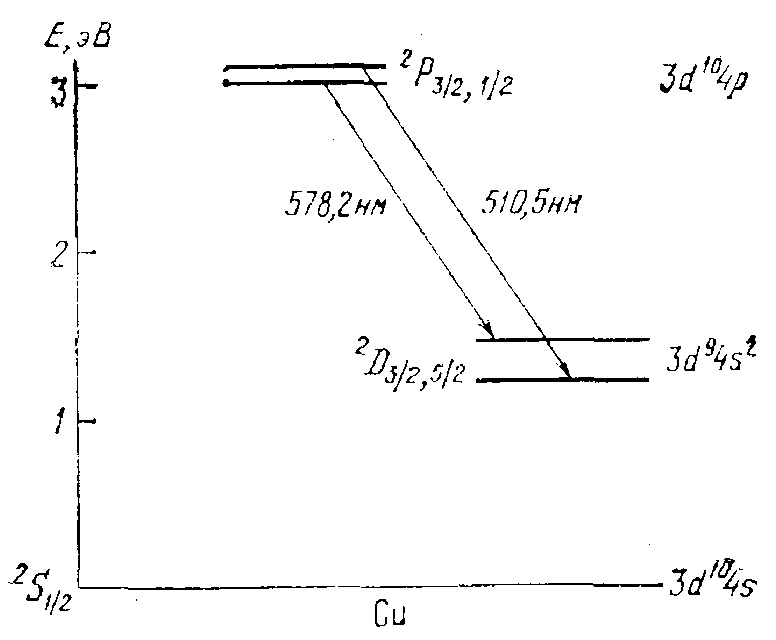
\includegraphics[width=.47\textwidth]{20}
    \caption{Уровни энергии}
\end{figure}
Рабочим веществом является пар нейтральных атомов меди. Генерация 
осуществляется на волнах \( 578,2~\text{нм} \) и, главным образом, 
\( 510,5~\text{нм} \) при переходах между уровнями конфигураций 
\( 3d^{10}4p \) и \( 3d^9s^2 \) атома меди. Верхние лазерные уровни 
\term{2}{P}{1/2,3/2} являются резонансными, а нижние \term{2}{D}{3/2,5/2} -- 
метастабильными. В результате инверсия в нём может существовать только в 
течение времени, малого по сравнению с временем жизни нижнего лазерного 
уровня. Этот лазер относится к лазерам на самоограниченных переходах, инверсия 
в нём создаётся газовым разрядом в смеси паров меди и буферного газа.

Генерация носит существенно импульсный характер. При скоростном импульсном 
разряде осуществляется режим включения усиления, в котором длительность 
импульса излучения может быть намного короче времени жизни верхнего уровня. 
Частота следования импульсов не может превышать величину, обратную времени 
жизни нижнего уровня.

Лазеры на самоограниченных переходах характеризуются высоким значением КПД 
перехода
\[
	\eta_\text{пр} =
    	\frac{g_\text{н}}{g_\text{н}+g_\text{в}}\frac{h\nu}{E_\text{в}}.
\]
У медного лазера он составляет 38\%.